\begingroup
	\pgfdeclarelayer{background layer}
	\pgfsetlayers{background layer,main}
	\tikzstyle{zero}=[circle,draw=black,fill=white,inner sep=0pt,minimum size=3.5mm]
	\tikzstyle{one}=[circle,draw=black,fill=black,inner sep=0pt,minimum size=3.5mm]
	\tikzstyle{two}=[circle,draw=black,fill=gray,inner sep=0pt,minimum size=3.5mm]
		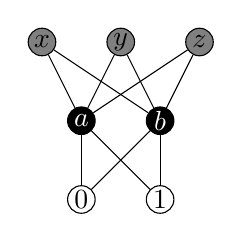
\begin{tikzpicture}
			\foreach \t in {1,2,3}
			{
				\ifnum \t<3
				\foreach \v/\l/\b in {1/0/a,2/1/b}
				{
					\ifnum \t=1
					\node (\l) at  (\v+.5,\t) [zero] {$\l$};
					\else
					\node [white] (\b) at (\v+.5,\t) [one] {$\b$};
					\fi
				}
				\else
				\foreach \v/\l in {1/x,2/y,3/z}
				{
					\node (\l) at (\v,\t) [two] {$\l$};
				}
				\fi
			}
			\foreach \x in {x,y,z}
			\foreach \l in {a,b}
			\draw[black] (\x)--(\l);
			
			\foreach \x in {0,1}
			\foreach \l in {a,b}
			\draw[black] (\x)--(\l);			
		\end{tikzpicture}
	%\label{fig:hasse_k_2_2_3}	
\endgroup